%% AI-based Village Pond Planning System — CSD Assignment 1, Final Technical Report.
%% Built on the course's acmart (manuscript, review) template. To use in Overleaf:
%% paste everything between \begin{document} and \end{document} into the template,
%% upload figures/ and refs.bib. Compile locally: `make report-latex`.
\documentclass[manuscript,review]{acmart}

\usepackage{algorithm}
\usepackage[noend]{algpseudocode}
\usepackage{tikz}
\usetikzlibrary{positioning,arrows.meta,fit,backgrounds}
\usepackage{tabularx}
\newcolumntype{L}{>{\raggedright\arraybackslash}X}

%% ---- one place for every link the report cites ---------------------------------
\newcommand{\repourl}{https://github.com/Rahul5977/AI-BasedPondAnalysis}
\newcommand{\appurl}{http://10.1.75.53:4270}
\newcommand{\videourl}{\textit{[YouTube link --- add after upload]}}

\setcopyright{acmlicensed}
\copyrightyear{2026}
\acmYear{2026}

\begin{document}

\title{AI-based Village Pond Planning System}
\subtitle{CSD Assignment 1 -- Final Technical Report}

\author{Rahul Raj}
\affiliation{%
  \institution{[Your Institute / Department]}
  \country{India}}
\email{rahul.raj9237@gmail.com}

\renewcommand{\shortauthors}{Rahul Raj}

\begin{abstract}
Village ponds harvest monsoon runoff, but siting one needs terrain, drainage, rainfall and
storage analysis that a Gram Panchayat rarely has. We built a web application in which an
administrator either draws a box around the village land on a satellite map or uploads a
KML/KMZ contour map, and receives a ranked pond location, the catchment draining to it, the
expected water volume and a costed pond design, all overlaid on the map. Elevation comes from
the upload (Delaunay TIN) or from the Copernicus GLO-30 DEM for the drawn box; both feed
one validated hydrology chain: Priority-Flood conditioning, D8 flow routing as a forest
of in-trees, a single topological sweep for accumulation and for a complete-catchment test,
multi-criteria site scoring with hard exclusions for rivers and mapped water, and catchment
delineation by reverse breadth-first search. Runoff is SCS-CN on 45 years of daily ERA5-Land
rainfall; the pond is sized by cost and checked by a daily water balance. Every number
carries a unit and an uncertainty band. The catchment engine matches the independent
pysheds implementation within 2--3\,\% on the same DEM; 219 tests (41 golden) pass;
46/46 end-to-end HTTP checks pass on the deployed lab VM. On one process a village-sized
selection is analysed in 2\,s (median) under 20 concurrent users.
\end{abstract}

\keywords{Village Pond Planning, Geospatial Analysis, Rainwater Harvesting, Catchment
Estimation, D8 Flow Routing, Web GIS, REST APIs}

\maketitle

%% =================================================================================
\section{Introduction}
Rural India stores monsoon water in small excavated ponds and tanks. A pond is only useful
where the terrain delivers enough runoff to fill it and not so much that the embankment
becomes a river dam. This report describes a system that finds such places from public
geospatial data and explains its answer. Section~\ref{sec:req} maps the requirements to
modules; Sections~\ref{sec:arch}--\ref{sec:method} give the high- and low-level design and the
algorithms (the examined core); Sections~\ref{sec:impl}--\ref{sec:csd} cover implementation
and the CSD themes; Section~\ref{sec:results} evaluates; Section~\ref{sec:limits} states the
limits.

\subsection{Motivation}
Selecting a site by hand needs a topographic survey, a rainfall record, a runoff estimate and
a storage calculation. Contour sheets are not digitised for most villages, rainfall gauges
are sparse, and land records are not public. The questions, however, are computable: where
does water converge, how much land drains there, how much rain falls in a normal (75\,\%
dependable) year, and what pond does that fill? An automated tool that answers them in
seconds, with stated uncertainty, lets an administrator shortlist sites before paying for a
survey.

\subsection{Scope of the Project}
\textbf{In scope:} selecting a land area on a map (a drawn box) or uploading a KML/KMZ
contour map; terrain products (DEM, slope, TWI, contours, streams); ranked pond sites with
per-criterion scores; catchment of any clicked point; 45-year rainfall statistics; runoff by
three methods; pond depth, dimensions, storage, fill reliability, spillway and indicative
cost; land-availability and water masks; saving, approving and exporting a recommendation.
\textbf{Out of scope:} structural design of the embankment, groundwater recharge modelling,
legal land ownership (never assumed; shown as unknown), and survey-grade accuracy --- all
results are planning grade from 30\,m public DEMs.

%% =================================================================================
\section{Problem Statement and Requirements}\label{sec:req}
The assignment asks for a web application that analyses terrain and rainfall to recommend
pond sites and estimates catchment, runoff, depth and storage on an interactive map. The
Phase~3 brief adds: select the land area on a map; return the suggested pond location,
catchment area and expected water volume for it, overlaid on the map; stay fast within the
four provided lab systems. Table~\ref{tab:fr} maps each requirement to its module.

\begin{table}[h]
  \caption{Functional requirements and where they are implemented}\label{tab:fr}
  \small
  \begin{tabularx}{\linewidth}{@{}lL@{}}
    \toprule
    Requirement & Implemented in \\
    \midrule
    Select land area on a map (Phase 3) & \texttt{web/src/components/AreaPanel.tsx}, \texttt{MapView.tsx}; \texttt{POST /analyzeArea}; \texttt{engines/terrain/adapters.py} (\texttt{ProviderTileAdapter}) \\
    Satellite imagery display & Esri World Imagery basemap in \texttt{MapView.tsx}; village named by reverse geocoding (\texttt{providers/geocoding.py}) \\
    Contour map visualization & \texttt{engines/terrain/contours.py} (marching squares + Douglas--Peucker); \texttt{GET /terrain/\{id\}/contours} \\
    Available-land identification & \texttt{engines/suitability/constraints.py} (Specification pattern), \texttt{water\_mask.py} (NDWI + OpenCV) \\
    Catchment area estimation & \texttt{engines/hydrology/\{conditioning,flow,catchment\}.py}; \texttt{POST /analysis/catchment} \\
    Suggested pond location & \texttt{engines/hydrology/siting.py} (MCDA + hard exclusions + NMS) \\
    Historical rainfall query & \texttt{providers/rainfall/} (Open-Meteo ERA5-Land, NASA POWER), \texttt{engines/rainfall/statistics.py} \\
    Runoff volume estimation & \texttt{engines/runoff/} (SCS-CN on the daily series, rational, Strange) \\
    Pond depth / storage recommendation & \texttt{engines/design/} (\texttt{PondDesignBuilder}, EAV, water balance, spillway) \\
    Combined overlay / results view & \texttt{web/src/components/ResultsOverlay.tsx} + map layers \\
    \bottomrule
  \end{tabularx}
\end{table}

\subsection{Non-Functional Requirements}
\textbf{Performance:} a village-sized area (0.25--25\,km$^2$) analysed end to end in under
10\,s; a catchment click under 2\,s. \textbf{Scalability and stress:} long work runs as
asynchronous jobs on bounded pools (bulkheads); a full queue answers \texttt{429} rather than
queueing without bound; request size is capped by area; replicas scale horizontally behind a
load balancer. \textbf{Availability:} external providers are wrapped in retry, circuit
breaker, cache and fallback; a dead replica is removed from rotation; the frontend works
offline from cache. \textbf{Correctness and honesty:} every number carries a unit and an
uncertainty band; warnings name every assumption. \textbf{Security:} JWT (RS256) with
viewer/planner/officer roles on the approval workflow; append-only audit log.
\textbf{Usability:} works on current Chrome/Firefox/Safari and at 390\,px width; Lighthouse
accessibility 100.

%% =================================================================================
\section{System Architecture and High-Level Design}\label{sec:arch}
The system is a layered monolith (ADR~0001) behind asynchronous job routes
(Figure~\ref{fig:arch}). The browser talks to one origin. The API validates and enqueues; a
worker runs the use-case workflow, which sequences pure engines and calls external data only
through adapters. Dependencies point inward only --- \texttt{api} $\rightarrow$
\texttt{engines} $\rightarrow$ \texttt{providers}/\texttt{repositories} $\rightarrow$
\texttt{domain} --- and a test (\texttt{tests/test\_layering.py}) fails the build if a router
holds business logic or an engine imports a framework.

\begin{figure}[h]
\centering
\begin{tikzpicture}[
  font=\scriptsize, node distance=3mm and 4mm,
  box/.style={draw, rounded corners=2pt, align=center, minimum height=7mm, inner sep=2pt, fill=white},
  ext/.style={box, fill=blue!6},
  store/.style={box, fill=orange!10},
  arr/.style={-{Stealth[length=1.6mm]}, thick}]
  \node[box, minimum width=28mm] (ui) {Browser SPA\\React + MapLibre\\draw box $\cdot$ upload $\cdot$ overlay};
  \node[box, right=6mm of ui, minimum width=26mm] (lb) {nginx\\\texttt{ip\_hash} load balancer\\(Docker: reverse proxy)};
  \node[box, right=6mm of lb, minimum width=30mm] (api) {FastAPI routers\\202 + job id $\cdot$ WebSocket\\JWT/RBAC $\cdot$ 429 backpressure};
  \node[box, below=5mm of api, minimum width=30mm] (wk) {Job workers (bulkheads)\\interactive $\mid$ heavy\\Celery or thread pools};
  \node[box, left=6mm of wk, minimum width=26mm] (wf) {Workflows\\contour/area analysis,\\catchment, runoff, design};
  \node[box, below=5mm of wf, minimum width=26mm] (eng) {Engines (pure numpy)\\terrain $\cdot$ hydrology $\cdot$ siting\\rainfall $\cdot$ runoff $\cdot$ design};
  \node[box, left=6mm of eng, minimum width=26mm] (dom) {Domain\\Quantity (value, unit, $\pm$)\\errors $\cdot$ GridSpec};
  \node[store, below=5mm of wk, minimum width=30mm] (db) {PostGIS $\cdot$ Redis $\cdot$ MinIO\\(lab: memory + local disk)};
  \node[ext, below=5mm of eng, minimum width=62mm, xshift=18mm] (prov) {Adapters: Copernicus GLO-30 (COG + water mask) $\cdot$ Open-Meteo / NASA POWER\\ESA WorldCover $\cdot$ SoilGrids $\cdot$ Sentinel-2 STAC $\cdot$ Nominatim};
  \draw[arr] (ui) -- (lb); \draw[arr] (lb) -- (api);
  \draw[arr] (api) -- (wk); \draw[arr] (wk) -- (wf); \draw[arr] (wf) -- (eng);
  \draw[arr] (eng) -- (dom); \draw[arr] (wk) -- (db); \draw[arr] (wf.south east) -- (prov.north);
  \draw[arr, dashed] (api.north) to[bend right=18] node[above, pos=.5]{result JSON, GeoJSON, progress} (ui.north);
\end{tikzpicture}
\caption{High-level system architecture. Arrows show the request path of an analysis: the
UI posts a box or a file, receives \texttt{202} with a job id, and follows progress over a
WebSocket (polling fallback) until the result is overlaid on the map.}\label{fig:arch}
\end{figure}

The same code runs in two shapes. The reference deployment is an 11-service Docker Compose
stack (PostGIS, Redis, MinIO, API, two Celery workers, beat, TiTiler, nginx + SPA,
Prometheus, Grafana). The four lab machines are unprivileged containers (no Docker, no
systemd, no root), so there each replica is one process with in-memory persistence, a
thread-pool job runner and a local object store, and replicas sit behind a user-space nginx
load balancer. The switch is configuration only: persistence, job runner and object store are
ports with two or three adapters each (ADR~0013).

\subsection{Technology Stack}
Python 3.12, FastAPI, Pydantic v2; numpy/scipy for every algorithm (no numba: at village
scale a legible sorted loop is fast enough); rasterio/GDAL for COG window reads and
reprojection; pyproj for UTM; OpenCV for the NDWI water mask; PostgreSQL + PostGIS,
Redis + Celery, MinIO; React + TypeScript + MapLibre GL; Docker Compose; GitHub Actions.
Elevation: the uploaded contour map, or Copernicus GLO-30 COGs~\cite{copdem} for a drawn box.
Rainfall: Open-Meteo ERA5-Land~\cite{era5land} with NASA POWER as fallback.
\textbf{Deviations from the suggested stack, justified:} FastAPI over Flask (typed OpenAPI
contract generated from the code, dependency injection for ports); PostgreSQL + PostGIS over
MongoDB (spatial types, boundary reuse by \texttt{ST\_Equals}, append-only audit rules in the
database); full DEM rasters over point-elevation APIs (flow direction needs a grid ---
a village is $\sim$10\,000 cells, one COG window read versus thousands of throttled point
calls); ERA5-Land over IMD (keyless, daily, 45 years in 2\,s; IMD gridded data needs
registration and manual download).

\subsection{Low-Level Design}
{\sloppy
\begin{itemize}
\item \textbf{Ports and adapters.} \texttt{DEMProvider} has two adapters:
  \texttt{ContourKMLAdapter} (parse, infer provenance, TIN) and \texttt{ProviderTileAdapter}
  (GLO-30 window read and warp). The analysis workflow's \emph{only} branch on input kind is
  which adapter to build. \texttt{JobRunner} has three (Celery, thread pools, inline for
  tests). Each rainfall provider is wrapped as \texttt{Cached(CircuitBreaker(Retry(p)))}
  inside a \texttt{FallbackChain}.
\item \textbf{Contract.} Every analysis route returns \texttt{JobAccepted\{job\_id,
  poll\_url\}}. Result schemas (\texttt{ContourAnalysisResult}, \texttt{CatchmentResult},
  \texttt{PondDesignResult}) are Pydantic models from which \texttt{openapi.json} and the
  frontend's TypeScript types are generated. Every numeric field is a \texttt{Quantity}
  \{value, unit, uncertainty\_pct, low, high, method\} --- a domain type, so a bare float
  cannot reach the API.
\item \textbf{Persistence of an analysis} is a Saga of four idempotent steps (village
  $\rightarrow$ rasters $\rightarrow$ streams $\rightarrow$ DEM asset) with compensations run in
  reverse on failure.
\item \textbf{Data model:} \texttt{villages} (PostGIS boundary), \texttt{dem\_assets}
  (provenance, statistics, object keys), \texttt{jobs} (status, stage, progress, result JSON,
  idempotency key), \texttt{recommendations} + outbox + append-only \texttt{audit\_log};
  rasters are Cloud-Optimised GeoTIFFs in the object store.
\end{itemize}\par}

%% =================================================================================
\section{Methodology}\label{sec:method}
Figure~\ref{fig:pipeline} (appendix) shows the pipeline; this section gives each stage.

\subsection{Terrain and Elevation Analysis}
\textbf{Map-selected area.} The box's centroid fixes the UTM zone; the grid is the envelope of
the projected box at GLO-30's native 30\,m. For every 1$^\circ$ tile the grid touches, the
window under the grid's own lon/lat footprint (plus two source cells) is read from the COG
over HTTP --- a few hundred kB --- and warped bilinearly onto the grid; tiles are mosaicked.
The tile's Water Body Mask (lake/river classes) is warped by nearest neighbour onto the same
grid. Limits of 0.25--25\,km$^2$, measured in metres, return \texttt{422 area\_out\_of\_range}
outside them.
\textbf{Uploaded contour map.} The KML/KMZ is parsed namespace-agnostically; elevation is
read by an ordered strategy (Z $\rightarrow$ whitelisted \texttt{ExtendedData} field
$\rightarrow$ placemark name), rejecting numeric \texttt{ID} decoys --- the provided sample
has one. Vertices are densified and triangulated (Delaunay TIN, linear interpolation,
Gaussian $\sigma$=1 cell). The cell size is derived, not configured: mean contour spacing
(hull area / total contour length) / 4, floored at the source DEM's resolution, which is
inferred from the file's own metadata (the sample: SRTM, 30\,m).
\textbf{Surfaces.} Slope, aspect and hillshade by Horn's 3$\times$3 kernel~\cite{horn1981};
profile and plan curvature~\cite{zevenbergen1987}; topographic wetness index
$\ln(a/\tan\beta)$~\cite{beven1979}; contours by marching squares, simplified by
Douglas--Peucker~\cite{douglas1973}. \textbf{OpenCV} builds the existing-water mask from
Sentinel-2 NDWI~\cite{mcfeeters1996}: Otsu threshold~\cite{otsu1979}, morphological
open/close, connected components with an area filter.

\subsection{Catchment Area Delineation}
\textbf{Conditioning.} Priority-Flood with $\varepsilon$~\cite{barnes2014,wang2006} fills
every depression to its spill level and gives flats a tiny gradient in one $O(n\log n)$ pass,
so every cell drains. \textbf{The flow graph.} D8~\cite{ocallaghan1984} gives each cell one
out-edge to its steepest-descending neighbour (diagonal drops divided by $\sqrt2$). Every
node has out-degree $\le 1$ and the filled surface has no cycles, so the graph is a forest of
in-trees rooted at map-edge outlets, and \emph{descending filled elevation is a topological
order}. One sorted sweep therefore computes flow accumulation (subtree size) and, with OR in
place of $+$, whether a cell's catchment reaches the map edge (Algorithm~\ref{alg:sweep}).
Streams are cells draining $\ge$\,5\,ha (an area, so it means the same at any resolution),
ordered by Strahler~\cite{strahler1957}.
\textbf{Delineation.} A click is snapped to the \emph{nearest} cell within 150\,m that drains
$\ge$\,2\,ha --- nearest, not largest, so a tributary click is not dragged onto the river ---
and the distance moved is shown. The catchment is the reverse breadth-first search from the
outlet over the inverted D8 edges (Algorithm~\ref{alg:bfs}); area, longest flow path (deepest
BFS level) and relief come from the same walk. Area uncertainty is
$\max(15\%,\ \text{one cell ring around the perimeter})$. \emph{Assumptions and limits:} D8
cannot split flow (D-$\infty$ is a documented stub); on very flat land a 2\,m DEM error can
redirect a small flow path (Section~\ref{sec:results}); the result is bounded by the selected
area --- hence the complete-catchment constraint below.

\begin{algorithm}[h]
\caption{One topological sweep: accumulation and edge-fed flags --- $O(n\log n)$}\label{alg:sweep}
\small
\begin{algorithmic}[1]
\Require filled DEM $z$, receiver $r(c)$ from D8 ($-1$ at outlets)
\State $acc(c)\gets 1$;\quad $edge(c)\gets [c$ on the grid border or beside nodata$]$ \textbf{for all} $c$
\For{$c$ \textbf{in} cells sorted by $z$ descending} \Comment{a topological order of the D8 forest}
  \If{$r(c)\ne -1$}
    \State $acc(r(c)) \gets acc(r(c)) + acc(c)$ \Comment{subtree size = upstream cells}
    \State $edge(r(c)) \gets edge(r(c)) \lor edge(c)$ \Comment{catchment reaches the map edge}
  \EndIf
\EndFor
\State \Return $acc \times$ cell area,\ $edge$
\end{algorithmic}
\end{algorithm}

\begin{algorithm}[h]
\caption{Catchment of a pour point --- reverse BFS, $O(\text{catchment size})$}\label{alg:bfs}
\small
\begin{algorithmic}[1]
\Require outlet $o$ after snapping; donor lists $D(c)=\{d : r(d)=c\}$ (inverse D8, built once)
\State $Q\gets[o]$;\ $seen\gets\{o\}$;\ $level(o)\gets 0$
\While{$Q$ not empty}
  \State $c\gets Q.\textsc{pop}()$
  \For{$d \in D(c)$}\ $seen\gets seen\cup\{d\}$;\ $level(d)\gets level(c)+\ell(d,c)$;\ $Q.\textsc{push}(d)$\EndFor
\EndWhile
\State \Return mask $seen$, area $|seen|\cdot$cell area, longest flow path $\max level$
\end{algorithmic}
\end{algorithm}

\subsection{Site Selection --- How the Area Is Chosen}
The suggested location is the best-scoring cell of the drainage network after \emph{hard
exclusions} (Algorithm~\ref{alg:site}). Scoring is a weighted sum of four memberships in
$[0,1]$ with weights from a Saaty pairwise matrix (principal eigenvector, consistency ratio
0.004~\cite{saaty1980}): \emph{upstream area} as a plateau in $\log_{10}$\,ha (0 at 1\,ha,
1 from 10 to 150\,ha, 0 at 1\,000\,ha --- enough to fill a pond, not a river), \emph{flatness}
(1 on 0--3\,\% slope, 0 at 15\,\%), \emph{wetness} (normalised TWI) and \emph{impoundment
efficiency} (volume held behind a nominal 2\,m rise by an 8-connected flood fill on the
upstream side, divided by its footprint --- natural basins score high). Exclusions come first
because a score cannot express ``never'': channels beyond 1\,000\,ha and mapped water are
rivers; nothing within a 200\,m flood belt of a channel beyond 150\,ha or of mapped water; and
nothing whose catchment reaches the map edge, because its area and runoff would be lower
bounds. Non-maximum suppression at 200\,m keeps the top five distinct.

\begin{algorithm}[h]
\caption{Pond site selection (terrain MCDA with hard exclusions)}\label{alg:site}
\small
\begin{algorithmic}[1]
\Require streams $S$, upstream area $A$, slope $s$, TWI, water mask $W$, edge-fed flags $E$
\State $river \gets (S \land A\ge 1000\,\text{ha}) \lor W$;\quad $major\gets (S\land A\ge 150\,\text{ha})\lor W$
\State $C\gets S \land (s\le 15\%) \land \lnot river \land \textsc{dist}(major) \ge 200\,\text{m}$ \Comment{distance transform}
\State \textbf{if} $C\land\lnot E\ne\emptyset$ \textbf{then} $C\gets C\land\lnot E$ \textbf{else} warn \texttt{no\_complete\_catchment}
\For{$c\in C$}\ $score(c)\gets\sum_k w_k\, \mu_k(c)$ \Comment{area plateau, flatness, TWI, impoundment}\EndFor
\State \Return top 5 by $score$ with non-maximum suppression (200\,m), each with its $\mu_k$
\end{algorithmic}
\end{algorithm}

\subsection{Rainfall Data Integration}
Daily precipitation 1981--2025 at the site from Open-Meteo's ERA5-Land archive, NASA POWER as
fallback, both behind retry, circuit breaker, a single-flight object-store cache and a
fallback chain that records which provider answered. Statistics use complete calendar years
only: mean, CV, \textbf{75\,\% dependable rainfall by the Weibull plotting position}
$P=m/(n+1)$ (the design year of Indian minor-irrigation practice), June--September share, IMD
rainy days ($\ge$\,2.5\,mm), and the 25-year 1-day depth by Gumbel EV1~\cite{gumbel1958}.

\subsection{Runoff and Pond Sizing}
Land cover from ESA WorldCover~\cite{worldcover} and soil texture from SoilGrids~\cite{soilgrids}
give an area-weighted TR-55 curve number~\cite{tr55}. SCS-CN
$Q=(P-0.2S)^2/(P+0.8S)$, $S=25400/CN-254$\,mm, is applied to \emph{each day} and summed ---
applied to annual totals it overestimates more than threefold (asserted by a test). The
rational coefficient and Strange's table~\cite{subramanya} bracket it; the spread is reported.
\textbf{Expected water volume} = 75\,\% dependable annual SCS-CN runoff $\times$ catchment area.
Design: target = runoff $\times$ 0.6 harvest efficiency, clamped to 2\,000--50\,000\,m$^3$; an
excavated frustum (2:1 sides, 0.5\,m freeboard) whose depth (1.5--3.5\,m) and aspect are chosen
by minimum cost; a daily water balance (inflow, evaporation, 2\,mm/day seepage) gives the
share of years the pond fills; the spillway passes the 25-year storm.

%% =================================================================================
\section{Implementation}\label{sec:impl}
\subsection{Backend and API Design}
REST under \texttt{/api/v1}, OpenAPI 3.1 generated from the code (Swagger at \texttt{/docs}).
Key routes:

\begin{center}\small
\begin{tabularx}{\linewidth}{@{}lL@{}}
\toprule
\texttt{POST /analyzeArea} & box $\rightarrow$ 202 job: site, catchment, terrain from GLO-30 \\
\texttt{POST /analyzeContour} & KML/KMZ (\texttt{contour\_map}) $\rightarrow$ 202 job, same result shape \\
\texttt{GET /jobs/\{id\}} $\cdot$ \texttt{WS /jobs/\{id\}/ws} & status, stage, percent \\
\texttt{GET /analysis/results/contour/\{job\}} & suggested location, rationale, catchment, 5 ranked sites, method \\
\texttt{POST /analysis/catchment} & catchment of any point (snap, BFS, metrics) \\
\texttt{GET /rainfall/statistics} & 45-year statistics at a point \\
\texttt{POST /analysis/runoff} $\cdot$ \texttt{/pond-design} & runoff range; full design with reliability and cost \\
\texttt{POST /analysis/suitability} & land constraints, NDWI water mask, AHP ranking \\
\texttt{GET /terrain/\{id\}/\{contours,streams,layers\}} & map layers \\
\texttt{/recommendations}, \texttt{/auth/token} & draft $\rightarrow$ submitted $\rightarrow$ approved (RBAC), audit, PDF/GeoJSON/CSV \\
\bottomrule
\end{tabularx}
\end{center}

Errors are RFC~9457 problem documents with stable codes generated from the same table the
handlers use (\texttt{GET /meta/errors}). Third-party failures degrade, never crash: rainfall
falls back provider $\rightarrow$ cache $\rightarrow$ recorded record; land cover and soil
fall back to stated defaults with a warning and a lower confidence label; an unreachable
water mask or geocoder is skipped and said so. Authentication: RS256 JWT, roles viewer,
planner, officer; approvals require officer.

\subsection{Frontend and Visualization}
A React + MapLibre single-page app (Figure~\ref{fig:ui}). \emph{Select land area}: search a
place, click two opposite corners; the box's area is checked live against the limits.
\emph{Analyse} posts the box, shows the job's stage and percentage, then draws the selected
area, contours with labels, streams by Strahler order, the five ranked sites, the top site's
catchment polygon and outlet, and --- after the pond design runs automatically on the top site
--- the pond footprint and a results overlay with location, catchment, 75\,\% rainfall, SCS-CN
runoff, storage, dimensions, fill reliability and a confidence badge. Any map click delineates
that point's catchment. Nineteen layers are toggleable; an offline-first service worker serves
cached results under an ``Offline'' badge.

\begin{figure}[h]
  \centering
  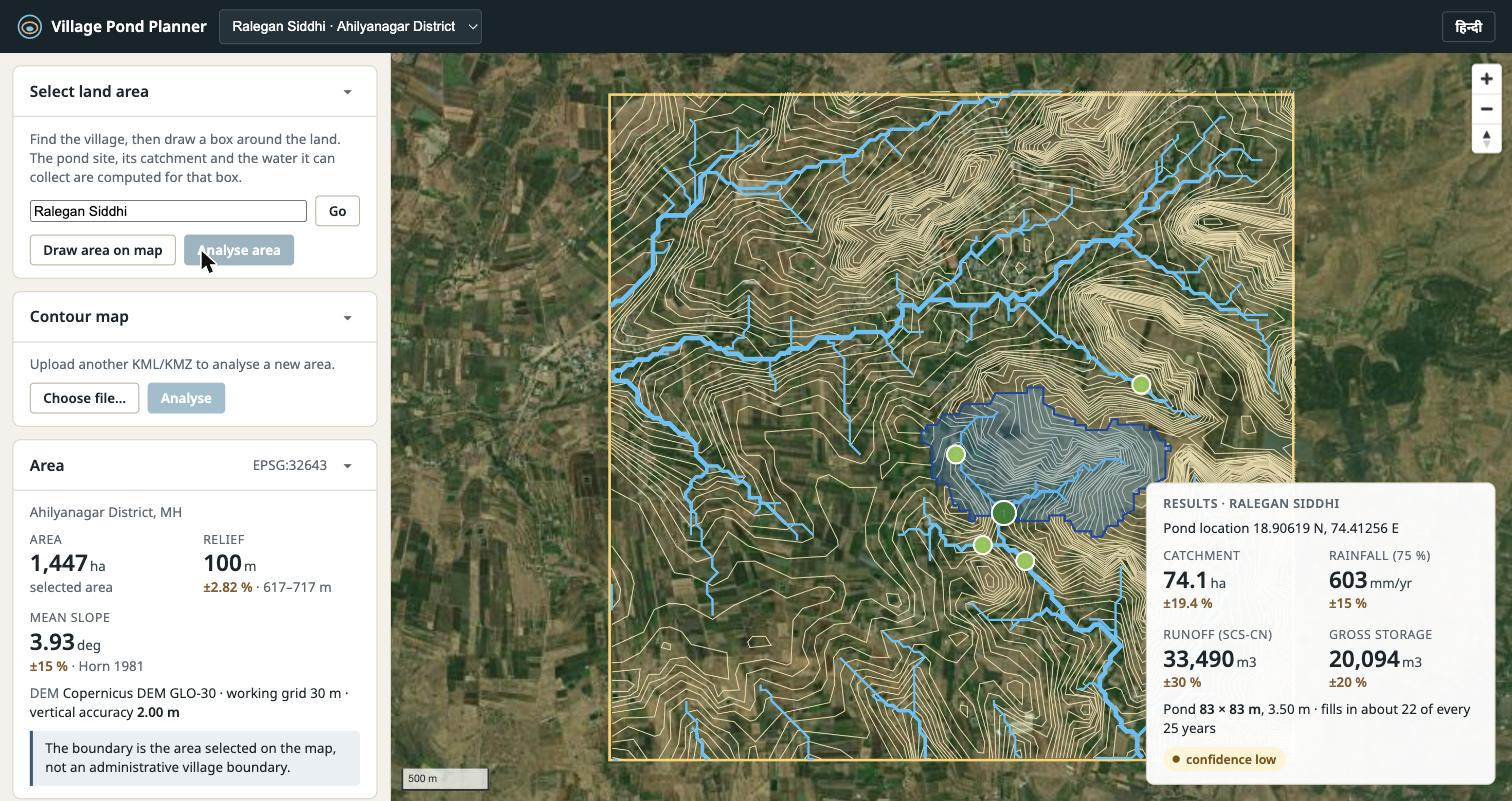
\includegraphics[width=\linewidth]{figures/p9-area-select.jpg}
  \caption{Application interface: a 14.5\,km$^2$ box drawn at Ralegan Siddhi (Maharashtra),
  analysed from Copernicus GLO-30 --- contours, streams, five ranked sites, the top site's
  74\,ha catchment and the results overlay (runoff 33\,490\,m$^3$, storage 20\,094\,m$^3$).}
  \label{fig:ui}
\end{figure}

\subsection{Database and Storage}
Villages with PostGIS boundaries (an identical boundary reuses the village), DEM assets with
provenance and statistics, jobs with idempotency keys, recommendations with a state machine
whose transitions write a transactional outbox drained into an \texttt{audit\_log} made
append-only by database rules. Rasters (DEM, slope, TWI, flow accumulation, \dots) are COGs in
MinIO served as tiles by TiTiler; streams and siting are JSON documents next to them; the
rainfall series is cached per point in the object store. On the lab VMs the same ports are
backed by memory and local disk.

%% =================================================================================
\section{CSD Themes and Topics Applied in the Project}\label{sec:csd}

\begin{table}[h]
\caption{Mapping of core CSD themes/topics to their use in this project}\label{tab:csd}
\scriptsize
\begin{tabularx}{\linewidth}{@{}>{\raggedright\arraybackslash}p{0.16\linewidth}LL@{}}
\toprule
CSD theme & Where used & Justification \\
\midrule
API design (REST) & \texttt{/api/v1}, 202 + job id, problem details, generated OpenAPI & long work must not hold a connection; clients branch on stable codes \\
Load balancing & nginx \texttt{ip\_hash} over four lab replicas, passive health checks & in-memory replicas need client affinity; a dead VM leaves rotation \\
Caching & single-flight rainfall cache; LRU GLO-30 windows; COG tiles; service worker & 45-year series once per point; a cold herd costs one upstream call \\
Indexing / query optimisation & PostGIS geometry, unique idempotency key, COG internal tiling & village reuse by boundary; byte-range reads of only the needed window \\
Concurrency / async & bulkhead pools (interactive, heavy), WebSocket progress, 429 backpressure & a village analysis cannot delay a click; bounded queues under stress \\
Microservices vs.\ monolith & layered monolith + workers & one team, one deployable; boundaries enforced by a test, not a network \\
Design patterns & Ports \& Adapters, Strategy, Decorator, Chain of Responsibility, Builder, Specification, Saga, State, Outbox, Observer & each solves a named problem (Section~\ref{sec:arch}) \\
AuthN / AuthZ & RS256 JWT, three roles, officer-only approval & approvals are accountable; audit log is append-only \\
Containerisation / deployment & Docker Compose (11 services); one-process replicas on the lab VMs & same code, two shapes, chosen by configuration \\
Error handling / resilience & retry, circuit breaker, fallback chain, stale cache, stated defaults & degrade with a warning rather than fail \\
Algorithms and complexity & Priority-Flood $O(n\log n)$, topological sweep $O(n)$, reverse BFS, distance transform & exact, textbook, explainable; $\sim$2\,s per village \\
Testing strategy & 219 tests: 41 golden (analytic terrain), API flows, pysheds cross-check, e2e over HTTP & hydrology correctness is checked against known answers \\
Version control / CI & conventional commits, GitHub Actions (ruff, mypy strict, pytest, image build) & every push proves the build \\
\bottomrule
\end{tabularx}
\end{table}

\textbf{Load balancing without shared state.} The lab VMs cannot run PostgreSQL or Redis for
this app, so replicas keep villages and jobs in memory; a user must keep reaching the replica
that ran their analysis. nginx \texttt{ip\_hash} gives that affinity, \texttt{max\_fails}
removes a dead replica and \texttt{proxy\_next\_upstream} retries on another --- the failover a
single VM cannot give (one lab VM's process died twice during the project). The cost is
stated: a failed-over user re-runs a 2\,s analysis. The Docker shape removes the limitation
with shared PostGIS/Redis/MinIO.
\textbf{Bulkheads over more threads.} The first lab load test showed \texttt{POST /analyzeArea}
blocking 11--21\,s: the inline runner ran the job inside the request. A thread-pool runner with
separate \emph{interactive} and \emph{heavy} pools returns \texttt{202} in milliseconds; the heavy
pool is deliberately small because the hydrology loops are GIL-bound Python --- more threads
would add waiting, not throughput; throughput comes from replicas.
\textbf{Single-flight caching.} Ten users opening the same village all missed the rainfall
cache and called Open-Meteo ten times (p95 43\,s). A per-key lock makes concurrent misses wait
for one upstream call (p95 63\,ms).

%% =================================================================================
\section{Results and Evaluation}\label{sec:results}
\textbf{Provided contour map} (Khapri, Durg, Chhattisgarh; 1\,355 contours, 267--298\,m, SRTM
30\,m source; UTM 44N derived from the file). The river entering from outside the map
(the Shivnath) carries no in-map accumulation, so an early version placed the top site on its
bank (Figure~\ref{fig:water}); with the water body mask, 92.7\,ha of water and its 200\,m belt
are excluded and the top site is a tributary (Figure~\ref{fig:results}): catchment
103\,ha\,$\pm$17\,\%, 75\,\% dependable rainfall 1\,192\,mm at the site (the overlay's
1\,151\,mm is the village-centroid series), CN 83, SCS-CN expected volume
172\,126\,m$^3$\,$\pm$30\,\% (rational 462\,k, Strange 49\,k: spread 182\,\%, reported), pond
50\,000\,m$^3$ (size cap binds), 126\,$\times$\,126\,m\,$\times$\,3.5\,m, fills in 25 of 25
years, INR 97 lakh indicative, confidence \emph{moderate} (\emph{low} when SoilGrids is
unreachable and the soil group is assumed).

\begin{figure}[h]
  \centering
  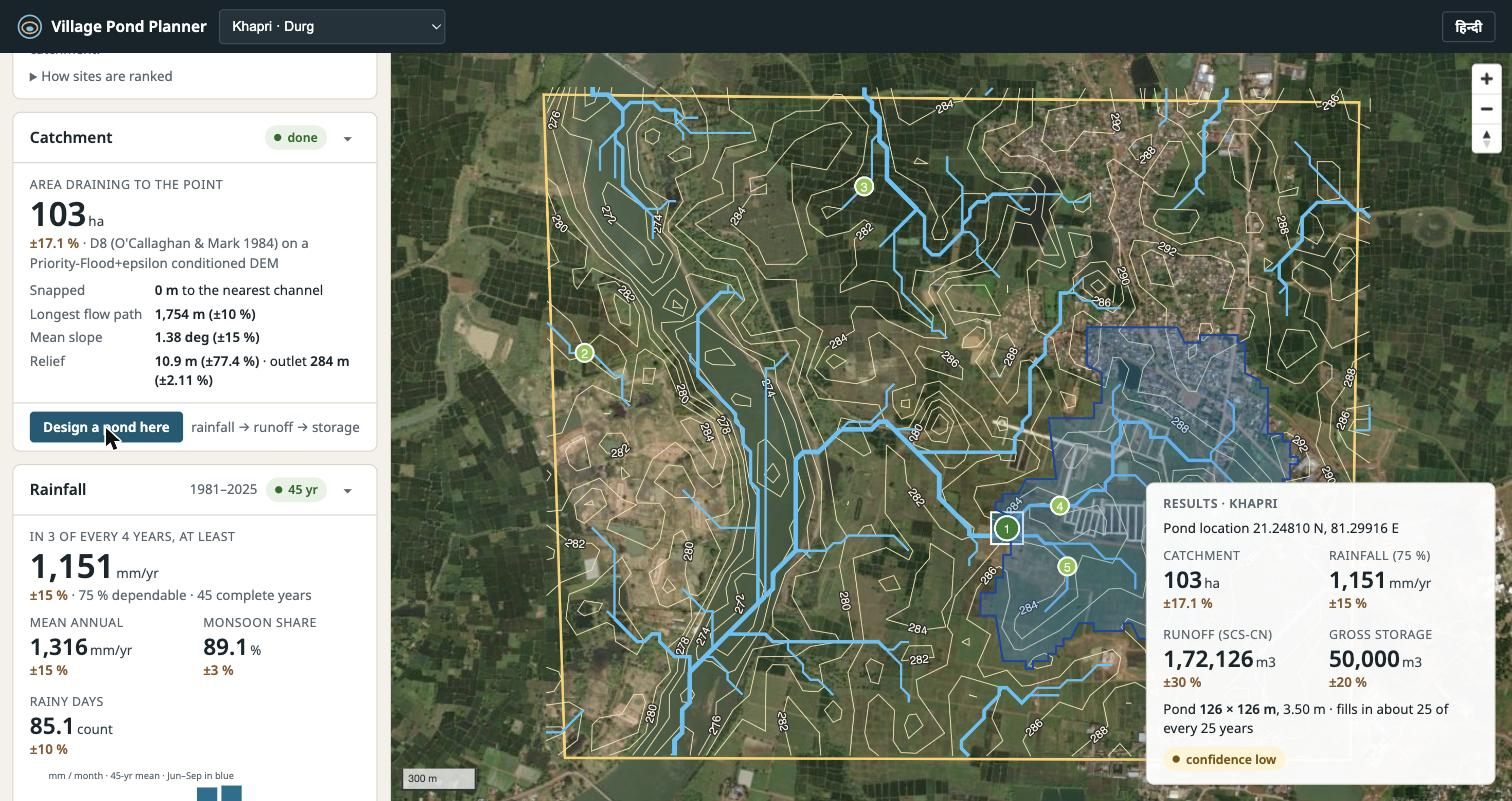
\includegraphics[width=\linewidth]{figures/p9-sample-results.jpg}
  \caption{Example results overlay for the provided contour map: ranked sites (all
  $\ge$\,295\,m from mapped water), the top site's 103\,ha catchment, and the pond result.}
  \label{fig:results}
\end{figure}

\textbf{Validation.} (i) 41 golden tests with analytic answers: inclined plane and cone
interpolation (RMS $<$0.25\,m), pit filling to spill level, plane accumulation equal to the
upslope cell count, V-valley catchment equal to the rectangle upstream, Y-valley Strahler
order 2, edge-fed flags on a hill and a tilted plane, river and water exclusion with the flood
belt, SCS-CN and frustum hand calculations. (ii) \textbf{Independent implementation:}
pysheds~\cite{pysheds} on the same DEM agrees within 2.0\,\% and 3.4\,\% on the main outlets
(22.5\,\% on a floodplain flat where flat-resolution schemes differ). (iii) \textbf{Independent
elevation source:} GLO-30 against the contour DEM on the sample --- surfaces agree (RMSE
1.8\,m after a $-$5\,m datum offset, $r$=0.94) but on this flat terrain (mean slope
1.6$^\circ$) small flow paths do not, and catchments at small sites differ several-fold
(Figure~\ref{fig:xcheck}); the algorithm is not the uncertainty, the source DEM is --- hence
the bands. (iv) Snapping cuts the pour-point coefficient of variation from 212\,\% to 48\,\%.
(v) The two OSM-mapped tanks in the sample are canal-fed; local runoff is a tenth of their
capacity --- recorded honestly as a mismatch of purpose, not of method.

\subsection{Performance}
Measured with Locust, 20 concurrent users (10 clicking catchments, 10 drawing a \emph{new} box
each time, so no cache helps), 90\,s, against one process (8-core laptop, thread-pool runner,
live GLO-30 and Open-Meteo): \texttt{POST
/analyzeArea} p95 17\,ms; full area analysis (GLO-30 read, hydrology, siting, catchment)
p50 2\,s, p95 4\,s, 154 analyses; catchment end to end p95 530\,ms; rainfall p95 63\,ms. Before
the bulkhead runner and single-flight cache the same test gave 11--21\,s and 43\,s. The
46-check end-to-end HTTP suite passes against the deployed lab replica. On the Docker stack,
50 users clicking catchments gave POST p95 33\,ms and end-to-end p95 560\,ms with no failures;
a catchment returned in 0.6\,s while a heavy suitability job ran (bulkheads).
\textbf{Limits within the four systems:} one process sustained 1.7 area analyses per second;
the 25\,km$^2$ cap bounds one request to seconds; \texttt{429} backpressure caps each queue at
20 jobs; replicas share nothing, so throughput should grow roughly linearly with the four
lab replicas behind the balancer (expected, not yet measured on the lab network).

%% =================================================================================
\section{Discussion and Limitations}\label{sec:limits}
\textbf{What worked:} one hydrology chain behind a DEM port served both the Phase~2 upload and
the Phase~3 map selection unchanged; every edge case found by looking at the map (a pond on
the river, a truncated catchment, a flattened river surface) became a hard rule with a golden
test and a named warning. \textbf{Limits:} both DEMs are 30\,m (SRTM $\pm$6\,m and GLO-30
$\pm$2\,m relative); relief below a few metres is not real, and on flat land the catchment of
a small site is dominated by DEM error --- the reason for the $\pm$15--50\,\% bands and the
advice to verify the outlet in the field. GLO-30 is a surface model (trees and buildings
included). Reanalysis rainfall is about $\pm$15\,\% against gauges. The three runoff methods
disagree by up to 2$\times$; SCS-CN is the design figure and the range is shown. Land
ownership is unknown without cadastral data and is never assumed. The ML scorer is deferred:
two mapped tanks are not a training set. Lab replicas keep state in memory, so a restart
forgets villages (re-analysis takes seconds).

%% =================================================================================
\section{AI Tool Usage Declaration}
An AI coding assistant (Claude Code, Anthropic) was used under the author's direction and
review, as the assignment's LLM policy permits, for: refactoring and structuring code into
the layered design; brainstorming and understanding the algorithms (D8 as a functional graph,
why descending elevation is a topological order, catchment as reverse BFS, the river and
truncation edge cases); implementing features to the author's specification with tests
alongside (including the map-selection adapter and the lab deployment); debugging defects
found by running the system; and editing this report and its figures, reformatting it into
this template. Every number in the report is produced by the code. Every design decision is
recorded with its reasoning and rejected alternatives in 21 architecture decision records and
the decision log (\texttt{docs/PROGRESS.md}); the author has reviewed, understood and can
explain each component.

\bibliographystyle{ACM-Reference-Format}
\bibliography{refs}

%% =================================================================================
\appendix
\section{Source Code and Repository}
\textbf{Repository:} \url{\repourl} (public). \textbf{Working front-end:} \url{\appurl}
(Swagger at \texttt{/docs}, planner at \texttt{/app}). \textbf{Demo video (5 min):} \videourl.
\textbf{Run anywhere:} \texttt{make up \&\& make seed} (Docker, 11 services) or
\texttt{make serve-single} (one process); \texttt{make check} runs lint, types and tests.
\textbf{Structure:} \texttt{app/} (\texttt{api} routers, \texttt{schemas}, \texttt{engines}
--- terrain, hydrology, rainfall, runoff, design, suitability, workflows ---, \texttt{domain},
\texttt{providers}, \texttt{repositories}, \texttt{jobs}), \texttt{web/} (React SPA),
\texttt{tests/} (incl.\ \texttt{golden/}), \texttt{infra/} (Compose, Dockerfiles, nginx, lab
replica script and load balancer), \texttt{docs/} (ADRs, API cookbook and error catalogue,
figures, progress log), \texttt{scripts/} (figures, cross-checks, e2e suite).

\clearpage
\section{Additional Figures}
\begin{figure}[h]
  \centering
  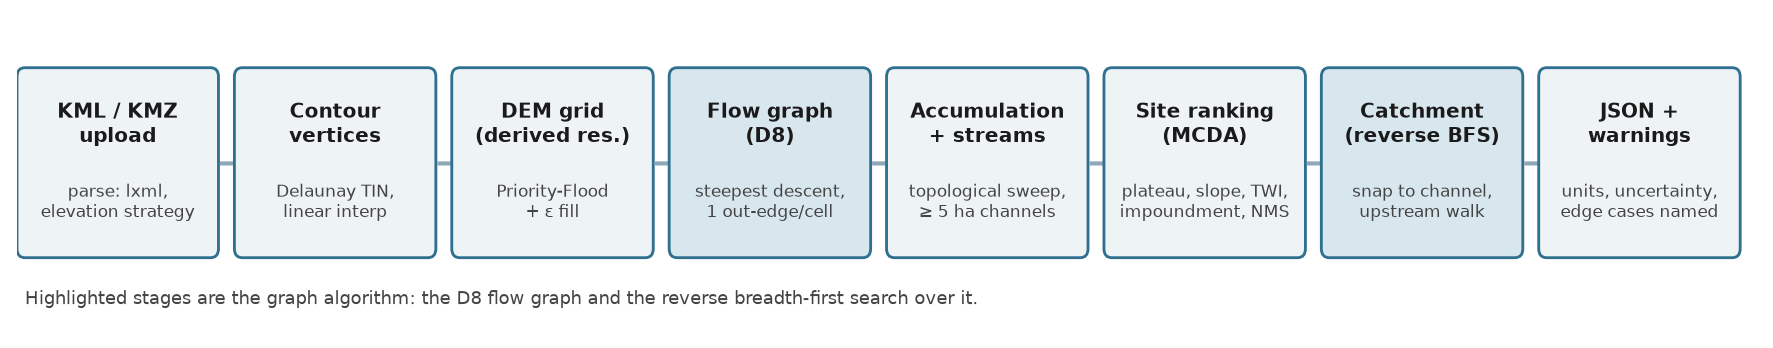
\includegraphics[width=0.9\linewidth]{figures/alg-pipeline.png}
  \caption{The analysis pipeline; the highlighted stages form the graph algorithm.}\label{fig:pipeline}
\end{figure}
\begin{figure}[h]
  \centering
  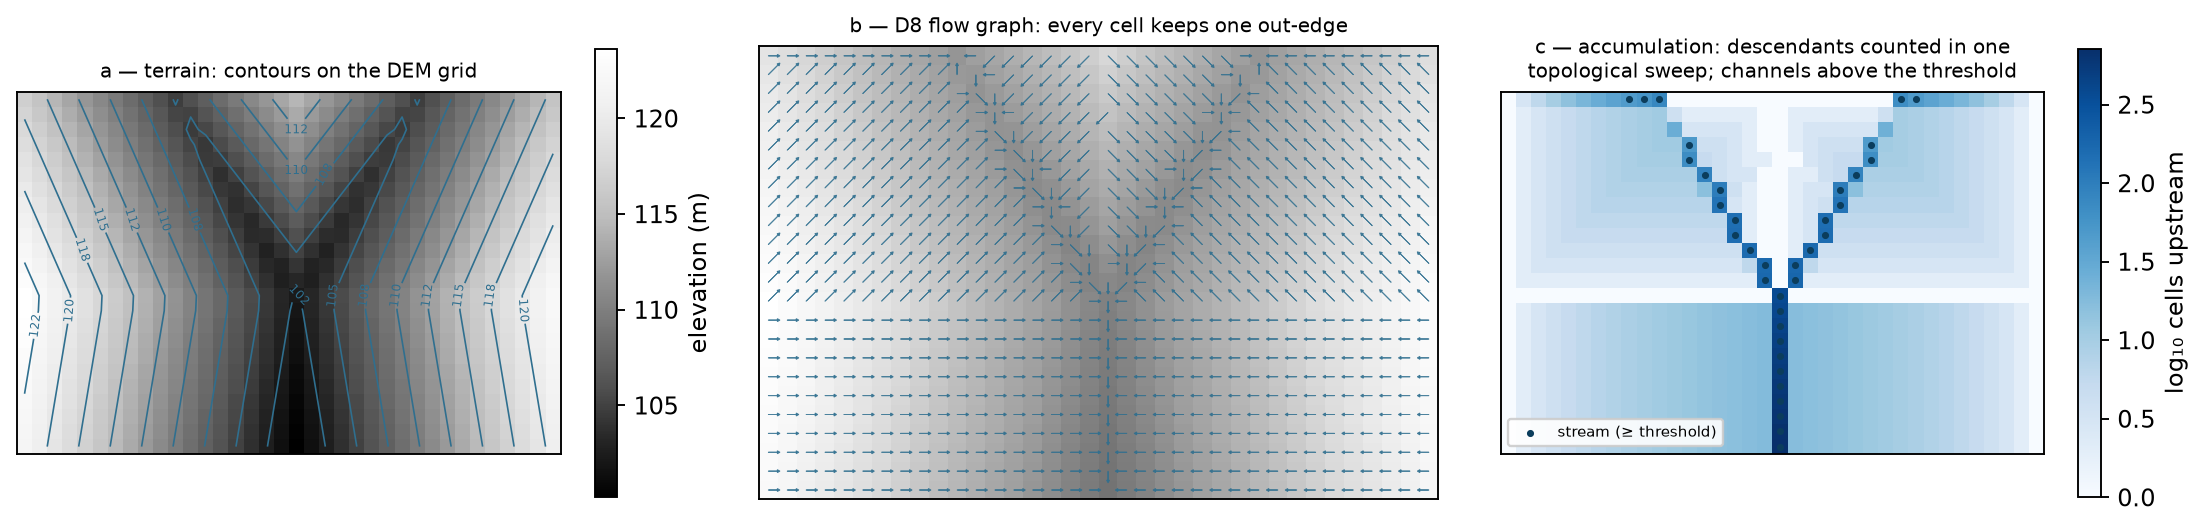
\includegraphics[width=\linewidth]{figures/alg-d8-graph.png}
  \caption{DEM $\rightarrow$ D8 flow graph $\rightarrow$ accumulation and streams (generated from the engine code).}
\end{figure}
\begin{figure}[h]
  \centering
  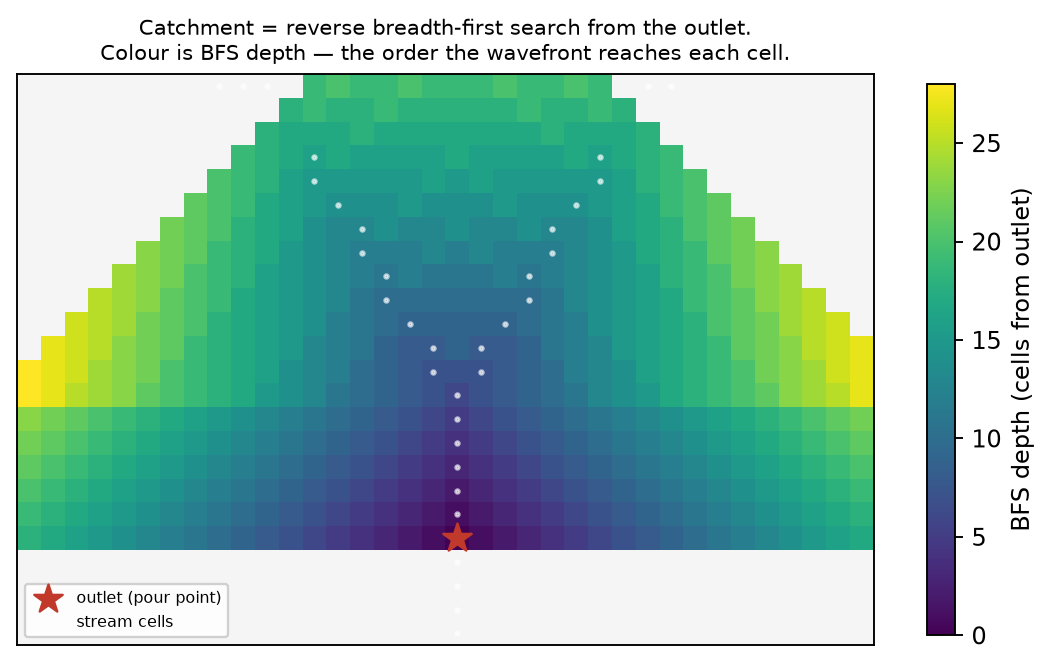
\includegraphics[width=0.75\linewidth]{figures/alg-catchment-bfs.png}
  \caption{Catchment as a reverse BFS from the outlet; colour is the wavefront order.}
\end{figure}
\begin{figure}[h]
  \centering
  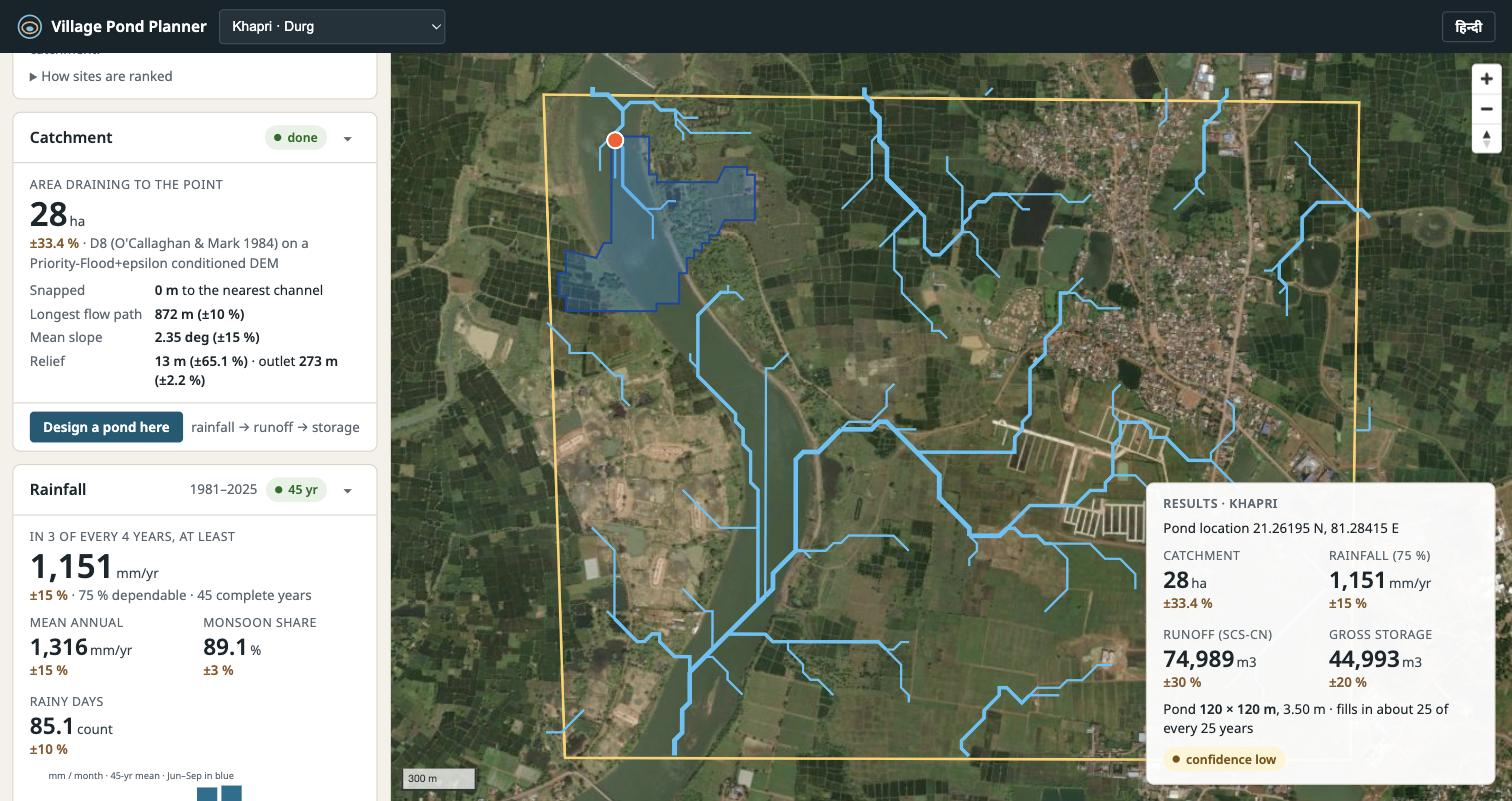
\includegraphics[width=0.85\linewidth]{figures/p9-watermask-before.jpg}
  \caption{Before the water body mask: the top site on the Shivnath's bank, its catchment
  40\,\% permanent water. Compare Figure~\ref{fig:results}.}\label{fig:water}
\end{figure}
\begin{figure}[h]
  \centering
  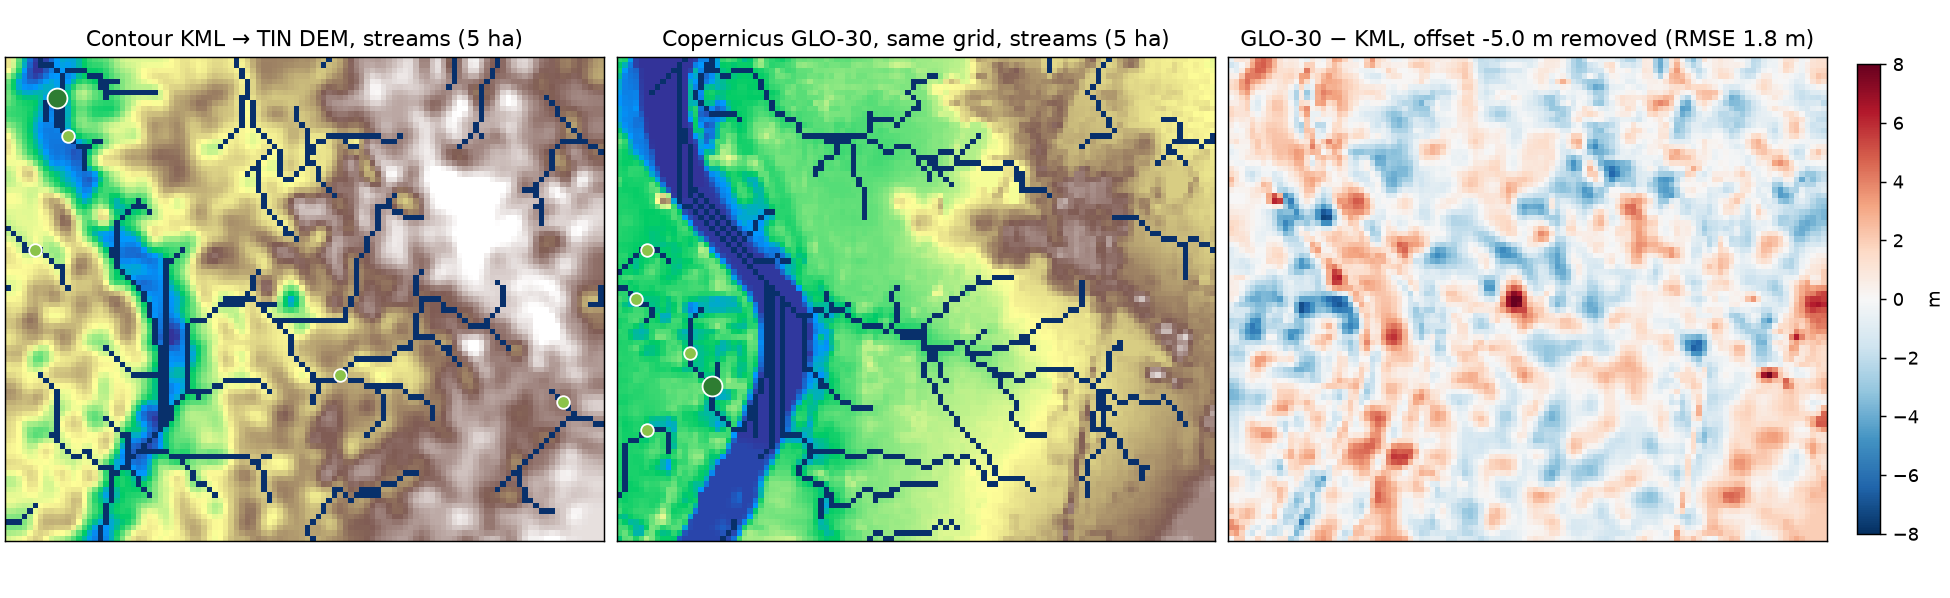
\includegraphics[width=\linewidth]{figures/p9-dem-crosscheck.png}
  \caption{Terrain-source cross-check on the sample: contour DEM vs.\ GLO-30 on the same grid,
  streams and sites from the identical chain, and the elevation difference.}\label{fig:xcheck}
\end{figure}
\begin{figure}[h]
  \centering
  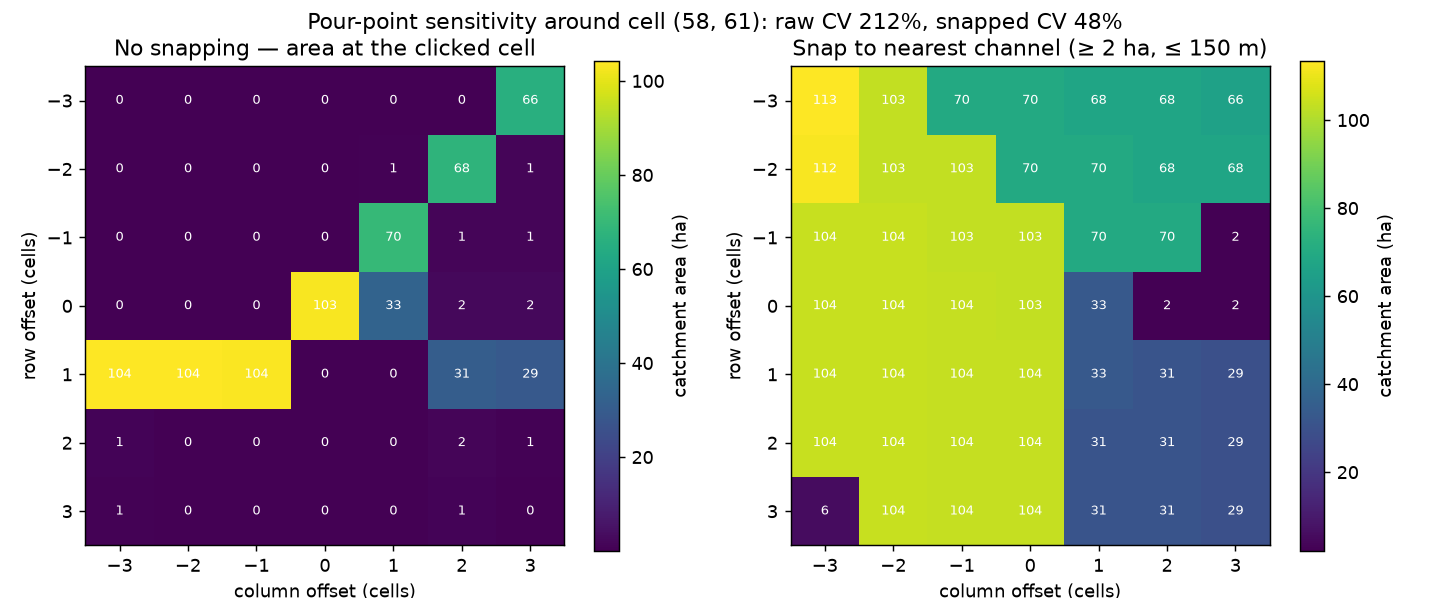
\includegraphics[width=0.85\linewidth]{figures/p2-pour-point-sensitivity.png}
  \caption{Pour-point sensitivity: catchment area around a channel cell, raw vs.\ snapped.}
\end{figure}
\begin{figure}[h]
  \centering
  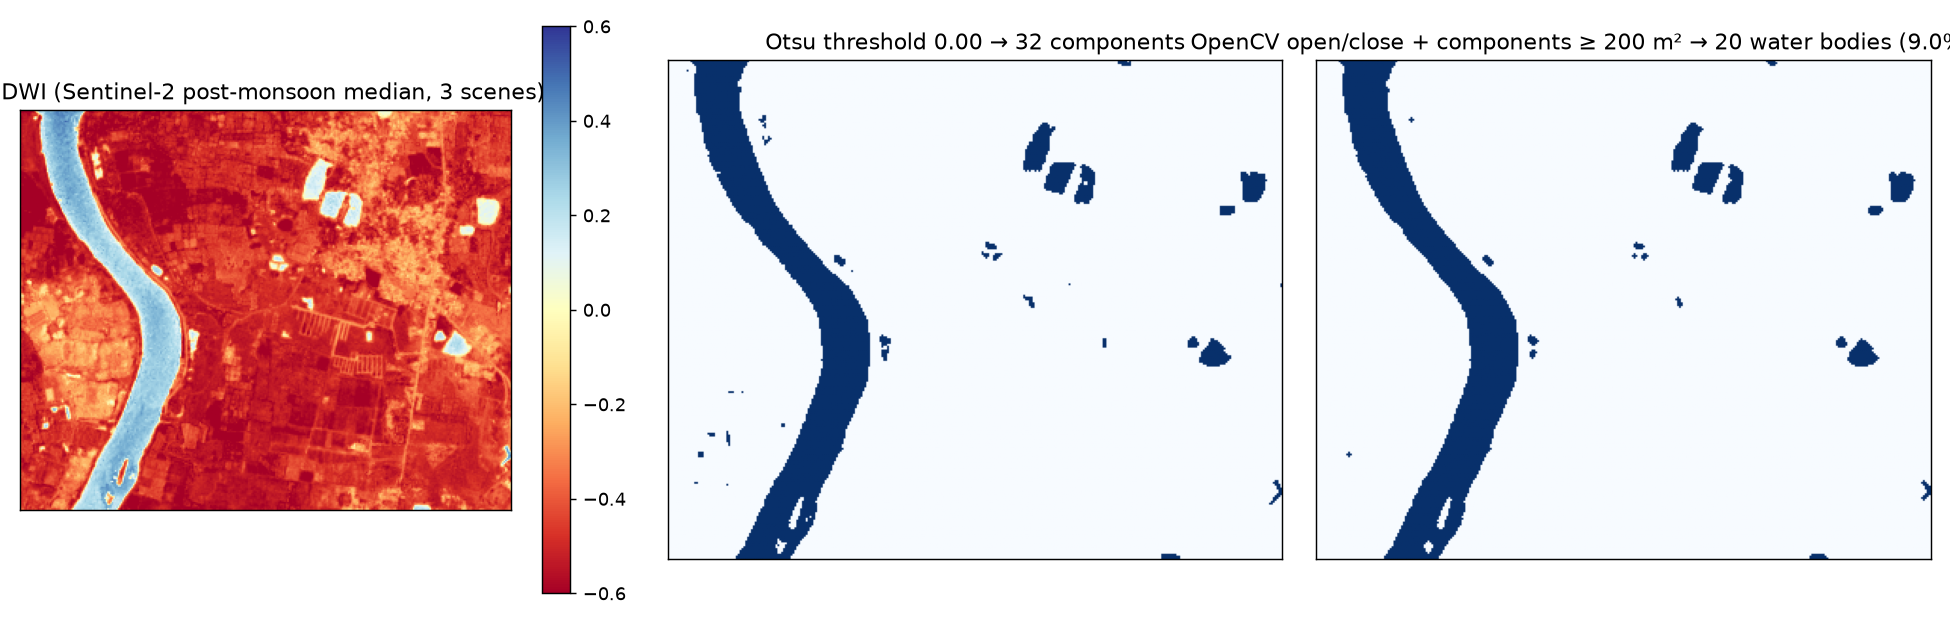
\includegraphics[width=0.85\linewidth]{figures/p4-ndwi-opencv.png}
  \caption{NDWI water mask with OpenCV: Otsu threshold, morphology, connected components.}
\end{figure}


\end{document}
